\subsection{Etudes aérodynamiques assistées par ordinateur (\acrshort{CFD})}

\subsubsection{Contexte et intérêt de la \acrshort{CFD}}

Afin de concrétiser ce projet, une étude aérodynamique approfondie par dynamique des fluides numérique a été menée. L’objectif
principal de l’étude est de valider théoriquement la faisabilité et l’efficacité du système d’aérofreins intégrés au premier
étage de la fusée, permettant de provoquer une augmentation contrôlée de la traînée et ainsi faciliter la séparation
avec le second étage.\\

Dans la mesure où l’expérience complète ne peut être validée uniquement par des essais expérimentaux (contraintes logistiques),
la \acrshort{CFD} est alors pour nous un outil indispensable permettant d’anticiper le comportement aérodynamique du système en
conditions de vol.\\

L’utilisation de la \acrshort{CFD} présente, pour ce projet, plusieurs intérêts majeurs comme le fait d’accéder à des grandeurs
aérodynamiques difficiles à mesurer expérimentalement sans l’utilisation de soufflerie. Cela concerne par exemple les champs de
pression et de vitesse ainsi que les efforts aérodynamiques localisés sur les aérofreins. L’approche \acrshort{CFD} nous permet
également de comparer quantitativement l’influence de différentes configurations d’ouverture des aérofreins qui, à partir des
données des simulations, permettent d’évaluer leur impact sur la trainée globale du premier étage. Elle offre aussi la
possibilité d’analyser le comportement de l’écoulement autour de la fusée, notamment le développement et le décollement de la
couche limite, phénomène acteur dans la génération de la trainée. Enfin, ces analyses fournissent une base théorique solide
permettant de justifier la pertinence du concept avant sa mise en œuvre au sein de l’association AéroIPSA.

\subsubsection{Stratégie de simulation}

Pour faciliter la réalisation des simulations \acrshort{CFD} et \acrshort{FEM}, une maquette numérique simplifiée de la fusée a
été développée à l’aide du logiciel de \acrshort{CAO} \acrshort{CATIA}. Cette maquette ne prend pas en compte certaines irrégularités
géométriques locales, telles que les sillons au niveau des trappes des parachutes ou les imperfections potentielles du tube en
fibre de verre et résine, inhérentes au procédé de fabrication.\\

Cette simplification géométrique a été volontairement adoptée afin de réduire la complexité du modèle numérique et, par
conséquent, les temps de calcul associés aux simulations, tout en conservant les caractéristiques aérodynamiques globales de la
fusée.\\

En effet, les irrégularités de faible amplitude n’ont qu’une influence négligeable sur les efforts aérodynamiques globaux
étudiés dans ce projet, comparativement aux effets induits par la géométrie générale et par le déploiement des aérofreins.
L’approche est cohérente avec la nature de l’étude qui vise à analyser le comportement aérodynamique global de la fusée, et non
les phénomènes locaux à très petite échelle ce qui nécessiteraient un modèle géométrique beaucoup plus détaillé.

\begin{figure}[H]
    \centering
    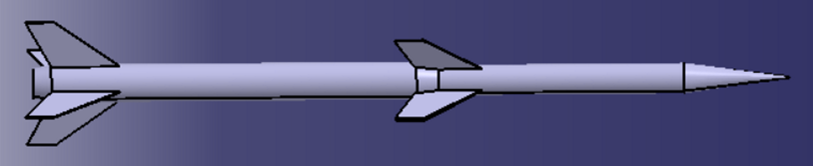
\includegraphics[width=0.9\linewidth]{figures/catpart_maquette.png}
    \caption{Maquette numérique simplifiée de la fusée (\acrshort{CATIA}).}
    \label{fig:catpart_maquette}
\end{figure}

À partir de la maquette numérique de la fusée, plusieurs configurations géométriques correspondant à différents degrés
d’ouverture des aérofreins ont été générées. Chaque configuration représente une position d’ouverture fixe des aérofreins et a
été exportée au format STEP (.stp), afin d’assurer leur compatibilité avec le logiciel de simulation \acrshort{CFD}. Les degrés
d’ouverture des aérofreins sont définis de manière paramétrique et exprimés en pourcentage, allant de 0 \%, correspondant à la
configuration aérofreins fermés, à 100 \%, correspondant à la configuration complètement ouverte. Cette discrétisation permet
d’étudier de manière l’influence de l’ouverture des aérofreins sur le comportement aérodynamique de la fusée (illustrations
présentées ci-après).


\begin{figure}[H]
    \centering
    \begin{subfigure}[b]{0.45\linewidth}
        \centering
        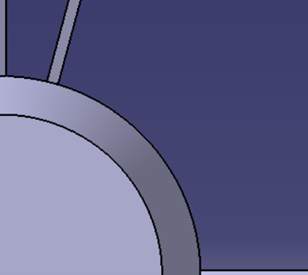
\includegraphics[width=\linewidth]{figures/AF0.png}
        \caption{Ouverture à 0 \% (fermés)}
    \end{subfigure}
        \hfill
    \begin{subfigure}[b]{0.45\linewidth}
        \centering
        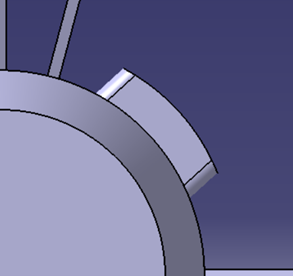
\includegraphics[width=\linewidth]{figures/AF50.png}
        \caption{Ouverture à 50 \%}
    \end{subfigure}
        \hfill
    \begin{subfigure}[b]{0.45\linewidth}
        \centering
        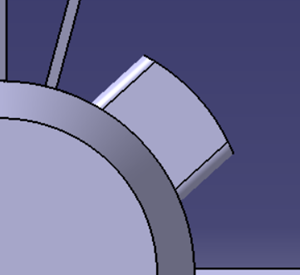
\includegraphics[width=\linewidth]{figures/AF100.png}
        \caption{Ouverture à 100 \% (ouverts)}
    \end{subfigure}
    \caption{Configurations d’ouverture des aérofreins étudiées.}
    \label{fig:af_configs}
\end{figure}

L’utilisation d’un pourcentage d’ouverture, plutôt que d’un angle absolu, permet de normaliser les configurations étudiées et de
nous faciliter lors de l’exploitation des résultats, notamment dans la recherche d’une loi reliant l’ouverture des aérofreins
aux efforts aérodynamiques générés. Les aérofreins sont considérés dans des positions fixes car l’étude ne porte pas sur la
phase transitoire d’ouverture ou de déploiement des aérofreins, mais sur les configurations stabilisées après déploiement.\\

Ce choix est motivé par le fait que la phase transitoire est de courte durée par rapport au temps de vol global ; la séparation
d’étages dépend principalement des efforts aérodynamiques une fois les aérofreins déployés et la modélisation du déploiement
nécessiterait un couplage avec une cinématique de structure. La prise en compte de positions fixes permet donc de dissocier les
effets aérodynamiques purs de la complexité mécanique du système.

\subsubsection{Hypothèses de modélisation}

Sur la base de cette maquette numérique, une stratégie \acrshort{CFD} a été élaborée afin d’analyser le comportement
aérodynamique de la fusée pour les différentes configurations. La simulation CFD a été définie en privilégiant un compromis
entre fidélité physique, robustesse numérique et exploitabilité des résultats. Les choix de modélisation présentés dans cette
section ont été effectués dans le but de fournir des résultats pertinents pour la validation théorique du système.\\

Les simulations ont été réalisées à l’aide du logiciel Simcenter STAR-CCM+, une plateforme de simulation d'ingénierie
multiphysique s’appuyant notamment sur la dynamique des fluides numérique. Largement utilisé dans les domaines de
l’aéronautique et du spatial, ce logiciel permet d’analyser des écoulements complexes et d’évaluer les performances
aérodynamiques de systèmes soumis à des conditions de vol réalistes.\\

Ici, le logiciel est utilisé pour déterminer, dans un premier temps, les efforts aérodynamiques globaux s’exerçant sur la fusée
et, dans un second temps, pour analyser plus spécifiquement les efforts induits par le déploiement des aérofreins.\\

La qualité des résultats fournis par une simulation \acrshort{CFD} dépend énormément des hypothèses de modélisation et des
modèles physiques. La section suivante présente les choix effectués pour la modélisation de l’écoulement.\\


\begin{minipage}{0.45\textwidth}
    \begin{itemize}
        \item \textbf{Three Dimensional : } Le calcul est réalisé en trois dimensions, ce qui permet de représenter fidèlement
        la géométrie complète de la fusée ainsi que les effets tridimensionnels de l’écoulement, notamment autour des
        aérofreins. Leur présence induit des phénomènes tridimensionnels (décollements, structures tourbillonnaires,
        dissymétries de l’écoulement). Une approche bidimensionnelle ou axisymétrique ne permettrait pas de capturer
        correctement ces effets.\\
        \item \textbf{Steady : } Le modèle Steady correspond à une résolution stationnaire des équations de l’écoulement,
        fournissant une solution indépendante du temps. L’objectif de l’étude est d’évaluer les efforts aérodynamiques moyens,
        en particulier la traînée, pour différentes configurations d’ouverture des aérofreins. Les fluctuations temporelles
        locales de l’écoulement ne sont pas étudiées ici. Ce choix permet d’obtenir une solution correcte à un coût de calcul
        réduit, cohérent pour une première validation théorique. Une approche instationnaire (unsteady) serait plus adaptée à
        l’étude du bruit, des vibrations ou du couplage fluide/structure, qui sortent du périmètre de ce travail.\\
    \end{itemize}
\end{minipage}
\hfill
\begin{minipage}{0.45\textwidth}
    \centering
    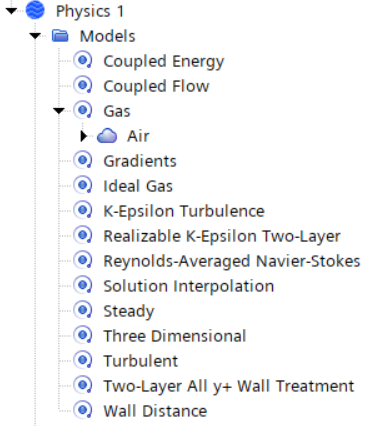
\includegraphics[width=\textwidth]{figures/propietes_model.png}
    \captionof{figure}{Propriétés physiques et modèles activés dans Simcenter STAR-CCM+.}
\end{minipage}

\begin{itemize}
    \item\textbf{Gas < Air : } Le fluide est modélisé comme un gaz, plus précisément de l’air, avec ses propriétés
    thermodynamiques standards pour une altitude donnée. Les simulations sont réalisées en conditions de vol atmosphérique.
    L’utilisation du modèle « Air » permet de représenter correctement la densité, la viscosité et les propriétés thermiques
    du fluide, nécessaires à la modélisation de la couche limite et des efforts aérodynamiques.\\
    \item \textbf{Ideal Gas : } Le modèle de gaz parfait relie pression, densité et température par l’équation d’état des
    gaz parfaits. À la vitesse considérée (191.9 m/s) et aux conditions atmosphériques étudiées, l’air peut être assimilé à un gaz
    parfait sans perte de précision significative. Ce modèle permet de prendre en compte les effets de compressibilité
    modérée tout en conservant une formulation simple et stable numériquement.\\
    \item \textbf{Reynolds-Averaged Navier–Stokes (RANS) : } Les équations de Navier–Stokes sont résolues sous leur forme
    moyennée de Reynolds, ce qui permet de modéliser les effets de la turbulence à l’aide de modèles statistiques. Comme
    l’écoulement autour de la fusée est majoritairement turbulent, une approche RANS permet de capturer les effets globaux
    de la turbulence (traînée, séparation de couche limite) à un coût de calcul compatible avec une étude paramétrique
    comportant plusieurs configurations d’aérofreins. Les approches LES (Large Eddy Simulation) ou DNS (Direct Numerical
    Simulation) seraient nettement plus coûteuses et non nécessaires pour l’analyse des grandeurs globales recherchées.
\end{itemize}

\newpage

\begin{figure}[h!]
    \centering
    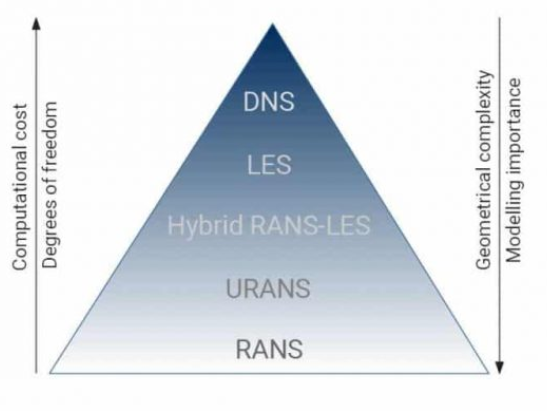
\includegraphics[width=0.8\linewidth]{figures/diagramme_des_methodes.png}
    \captionof{figure}{Comparaison qualitative des méthodes DNS, LES et RANS selon le coût de calcul et la précision.}
    \label{fig:diagramme_des_methodes}
\end{figure}

\begin{itemize}
    \item \textbf{Turbulent : } Ce modèle active la résolution d’un écoulement turbulent. Le nombre de Reynolds associé à
    l’écoulement autour de la fusée est élevé, ce qui implique un régime d’écoulement turbulent. Une hypothèse laminaire serait
    physiquement incorrecte et conduirait à une sous-estimation importante de la traînée.\\
    \item \textbf{K-Epsilon Turbulence \& Realizable K-Epsilon Two-Layer : } Le modèle $k-\varepsilon$ réalisable est un modèle de
    turbulence à deux équations qui résout l’énergie cinétique turbulente (k) et son taux de dissipation ($\varepsilon$). La
    formulation realizable améliore la cohérence physique du modèle, notamment dans les zones de fort cisaillement et de
    recirculation. L’approche Two-Layer permet une meilleure modélisation de la turbulence à proximité des parois. Ce modèle est
    particulièrement bien adapté aux écoulements externes aérodynamiques, avec la séparation de couche limite, le sillage
    développé et les gradients de pression importants induits par les aérofreins. Ce modèle offre un bon compromis entre
    précision et robustesse numérique, ce qui est essentiel dans une étude comparative portant sur plusieurs configurations.\\
    \item \textbf{Two-Layer All  Wall Treatment : } Ce traitement de paroi adapte automatiquement la modélisation de la turbulence
    en fonction de la valeur de, permettant une transition continue entre une résolution proche paroi fine et une approche par
    lois de paroi. La présence des aérofreins impose des variations locales importantes de la couche limite. Ce modèle permet de
    garantir une modélisation cohérente des efforts de frottement et de pression, même en présence de variations de raffinement
    du maillage.\\
    \textbf{Coupled Flow \& Coupled Energy : } Ces modèles assurent un couplage fort entre les équations de conservation de la
    masse, de la quantité de mouvement et de l’énergie. Bien que les effets thermiques ne soient pas prépondérants dans cette
    étude (subsonique), le couplage permet de prendre en compte les effets de compressibilité de l’air de manière cohérente,
    améliorant la stabilité et la précision de la solution à des vitesses subsoniques élevées.\\
    \item \textbf{Gradients : } Ce modèle permet le calcul précis des gradients des grandeurs physiques (vitesse, pression,
    turbulence). Les gradients sont essentiels pour le calcul des contraintes visqueuses, la modélisation de la turbulence et
    l’évaluation correcte des forces aérodynamiques.\\
    \textbf{Solution Interpolation : }Ce modèle définit la méthode d’interpolation des variables aux interfaces des cellules du
    maillage. Une interpolation appropriée permet d’améliorer la stabilité numérique et la précision de la solution, en
    particulier dans les zones de forts gradients autour des aérofreins.\\
    \textbf{Wall Distance : } Ce modèle calcule la distance minimale entre chaque cellule fluide et les parois solides. La
    distance à la paroi est une donnée clé pour le calcul de $y^{+}$, l’application correcte des lois de paroi et la modélisation
    de la couche limite.
\end{itemize}

\subsubsection{Modélisation de la géométrie et du maillage}
Pour le dimensionnement du domaine d’étude, il a été défini de manière à représenter un écoulement d’air libre autour de la fusée en limitant l’influence des conditions aux limites sur les résultats, c’est pourquoi il est modélisé sous la forme d’un domaine cylindrique de 14 mètres de longueur et de 4 mètres de rayon, au centre duquel est positionnée la fusée. Ces dimensions sont suffisamment grandes afin de garantir que les perturbations de l’écoulement induites par la fusée, et en particulier par le déploiement des aérofreins, se dissipent avant d’atteindre les frontières du domaine. Cette approche permet d’éviter toute interaction entre le sillage aérodynamique et les conditions aux limites, ce qui pourrait fausser l’évaluation des efforts aérodynamiques. La décision du domaine cylindrique permet aussi une représentation efficace de l’écoulement externe tout en limitant le volume total du domaine, et donc le coût numérique associé aux simulations.

\begin{figure}[H]
    \centering
    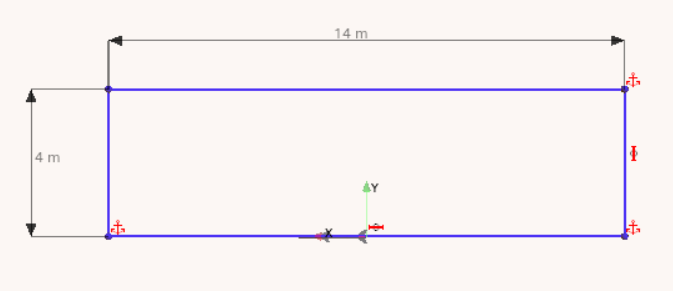
\includegraphics[width=0.9\linewidth]{figures/Sketch_geometrie.png}
    \caption{Schéma de la géométrie du domaine d’étude et des dimensions principales.}
    \label{fig:sketch_geometrie}
\end{figure}

\begin{figure}[H]
    \centering
    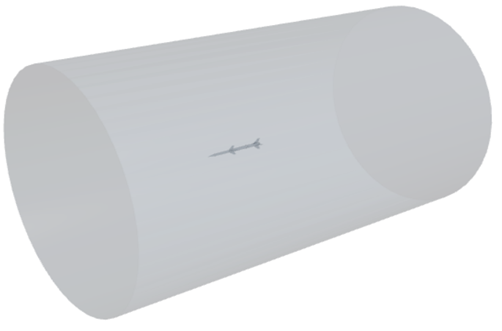
\includegraphics[width=0.9\linewidth]{figures/Representation_3D_domaine.png}
    \caption{Représentation 3D du domaine de calcul autour de la fusée.}
    \label{fig:representation_3d_domaine}
\end{figure}

\newpage

\begin{minipage}{0.55\textwidth}
    Une fois le domaine de calcul défini, une attention particulière a été portée à la stratégie de maillage, notamment à
    proximité de la fusée et des aérofreins. Le maillage a été généré à l’aide de l’outil Automated Mesh pour combiner un
    maillage volumique tétraédrique et un raffinement local adapté aux zones comme les aérofreins et les ailerons. Le but est
    d’obtenir une résolution suffisante des phénomènes physiques tout en limitant le nombre total de cellules afin de maintenir
    des temps de calcul raisonnable avec les plusieurs configurations d’ouverture. Le maillage final comporte 4 573 977
    cellules, ce qui permet de capturer correctement les gradients d’écoulement au voisinage de la fusée et des aérofreins.\\
    
    Le domaine de calcul représentant un écoulement d’air libre, aucune couche limite n’a été appliquée sur la surface du domaine
    cylindrique. Celui-ci ne constitue pas une paroi physique, mais uniquement une frontière délimitant l’environnement fluide,
    justifiant l’absence de raffinement particulier à proximité de cette surface. Pour adapter le maillage aux différentes
    parties du système, l’utilisation de l’outil Custom Controls a été nécessaire. Cette approche permet de concentrer la
    densité de maillage sur les zones où les gradients de vitesse et de pression sont les plus importants, tout en conservant
    un maillage plus grossier dans les régions moins intéressantes.
\end{minipage}
\hfill
\begin{minipage}{0.39\textwidth}
    \centering
    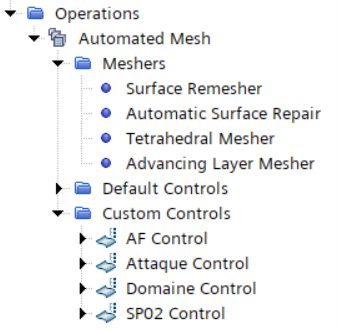
\includegraphics[width=\linewidth]{figures/configuration_du_mesh.png}
    \captionof{figure}{Configuration du maillage dans STAR-CCM+ (outil de maillage et contrôles).}
    \label{fig:configuration_du_mesh}
\end{minipage}

\vspace{1cm}

Le domaine fluide a un maillage volontairement plus grossier à distance de la fusée pour réduire significativement le nombre de
cellules car ce sont des zones où l’écoulement est peu perturbé.\\

Les aérofreins et les ailerons ont des géométries fines par rapport aux dimensions globales de la fusée mais elles jouent un
rôle central dans la génération de traînée. Un raffinement local du maillage a donc été appliqué sur ces éléments afin de
représenter correctement leur influence sur l’écoulement.

\begin{figure}[H]
    \centering
    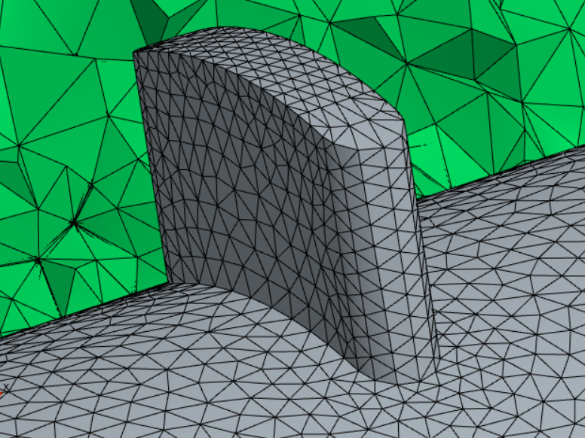
\includegraphics[width=0.8\linewidth]{figures/maillage_AF.png}
    \caption{Raffinement local du maillage au niveau des aérofreins.}
    \label{fig:maillage_af}
\end{figure}

\newpage

Le minimum surface size a été défini de manière à correspondre à la moitié de l’épaisseur locale de ces surfaces pour garantir
la présence d’au moins deux cellules à travers l’épaisseur. Cela est nécessaire pour assurer une représentation numérique
correcte de ces éléments minces.

\begin{figure}[H]
    \centering
    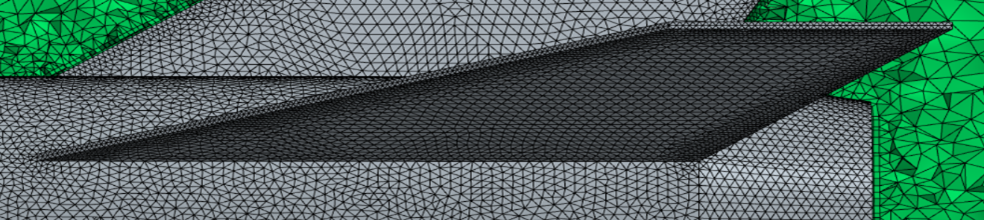
\includegraphics[width=0.9\linewidth]{figures/maillage_aileron.png}
    \caption{Raffinement local du maillage au niveau des ailerons.}
    \label{fig:maillage_aileron}
\end{figure}

SP02 Control

Un contrôle spécifique a également été appliqué à certaines surfaces via le SP02 Control, afin d’améliorer la représentation de
la courbure géométrique. Ce raffinement permet une meilleure approximation des surfaces courbes de la fusée et des aérofreins,
ce qui est essentiel pour une évaluation des champs de pression et des efforts aérodynamiques.

\begin{figure}[H]
    \centering
    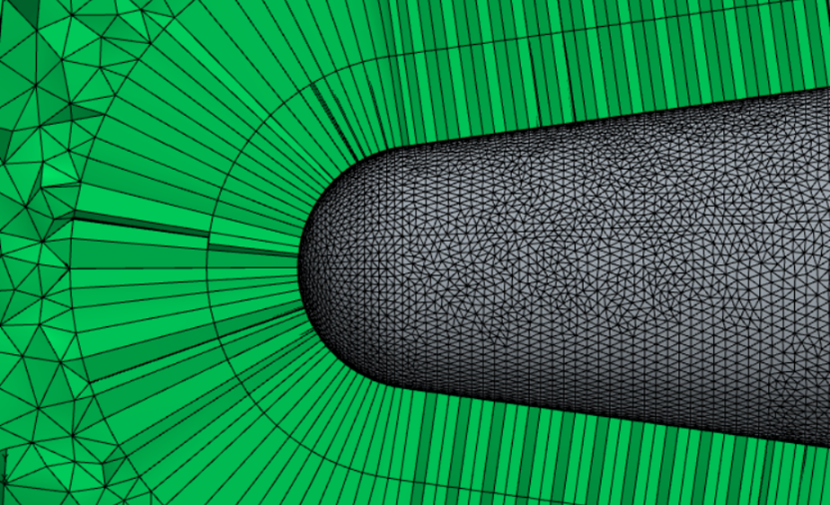
\includegraphics[width=0.9\linewidth]{figures/maillage_pointe.png}
    \caption{Maillage au niveau de la pointe de la fusée.}
    \label{fig:maillage_pointe}
\end{figure}

Pour limiter les variations brutales de taille de maille, le Surface Growth Rate a été fixé à 1,15, permettant une transition
progressive entre les zones fortement raffinées et les zones plus grossières. Cette approche assure que les résultats obtenus
sont principalement gouvernés par la physique de l’écoulement avec une résolution fine des aérofreins, ailerons et à la
proximité de la fusée. Une réduction du coût numérique dans les régions éloignées de l’objet et une bonne qualité des
cellules, garantissant la stabilité et la convergence des simulations \acrshort{CFD}. L’utilisation de contrôles de maillage
personnalisés permet ainsi d’optimiser la répartition des cellules au sein du domaine de calcul, en concentrant la résolution
là où elle est nécessaire pour l’analyse aérodynamique, tout en maintenant des temps de calcul compatibles avec les objectifs
du projet.

\begin{figure}[H]
    \centering
    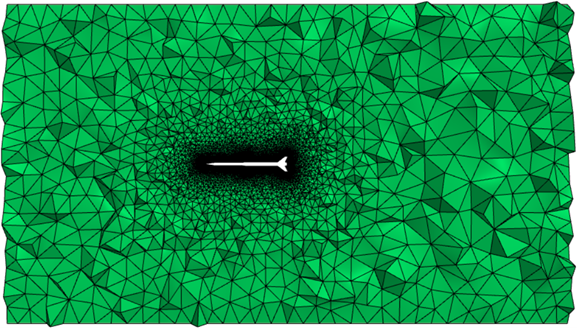
\includegraphics[width=0.9\linewidth]{figures/maillage_global_domaine.png}
    \caption{Vue globale du maillage du domaine de calcul.}
    \label{fig:maillage_global_domaine}
\end{figure}

\subsubsection{Résultats attendus}
En ce qui concerne les résultats attendus, les simulations \acrshort{CFD} vont permettre de mettre en évidence plusieurs
éléments physiques.\\

Tout d’abord, une augmentation du coefficient de traînée de la fusée est à envisagée à mesure que l’ouverture des aérofreins
augmente. Cette évolution est directement liée à l’accroissement de la surface exposée et à la modification du champ de
pression induite par ce déploiement des aérofreins. Au même moment, une augmentation des niveaux de pression sur les surfaces
des aérofreins est attendue pour chaque gradient d’ouverture. Cette augmentation de la pression est le principal élément à la
génération de traînée et joue donc un rôle déterminant dans l’efficacité du système des AF. L’analyse de l’écoulement devrait
également mettre en évidence des perturbations du flux au voisinage des aérofreins, telles que des zones de décollement de la
couche limite, des régions de recirculation et un élargissement du sillage en aval de la fusée. Ces phénomènes sont
caractéristiques des écoulements externes autour de corps équipés de dispositifs de freinage aérodynamique.\\

Enfin, en dehors des zones directement affectées par les aérofreins, l’écoulement autour de la fusée devrait conserver un
comportement aérodynamique classique, avec le développement d’une couche limite le long du corps. L’ensemble de ces éléments
permettra de vérifier la cohérence physique des résultats obtenus et de valider la capacité des simulations à représenter
correctement l’effet des aérofreins sur le comportement aérodynamique global de la fusée.

\newpage